\documentclass[11pt]{article}

%\usepackage[utf8]{inputenc}
\usepackage{indentfirst}
\usepackage[hidelinks]{hyperref}
\usepackage{float}
\usepackage{array}
\usepackage{listings}
\usepackage{csquotes}
\usepackage{enumitem, amsmath, amssymb, amsfonts, latexsym, mathrsfs}
\usepackage{graphicx}
\usepackage{subfig}
%\usepackage[greek,english]{babel}
%\usepackage{alphabeta}
\usepackage{multicol}
\usepackage{bookmark}

\usepackage{caption}
\captionsetup[figure]{font={small},labelfont={bf},justification={raggedright},singlelinecheck={false},name={Figura.}}

\usepackage{blindtext}

\usepackage{biblatex}
\addbibresource{bibliography.bib}

\usepackage[a4paper, total={6in, 8in}]{geometry}

% Setup de hiperenlaces
\hypersetup{
    colorlinks=true,
    linkcolor=cyan,
    filecolor=magenta,      
    urlcolor=cyan,
    pdftitle={Jiménez_Montero_Jesús_Crying_Girl_in_the_Border},
    pdfpagemode=FullScreen,
}

% Tipografía
\usepackage{helvet}
\renewcommand{\familydefault}{\sfdefault}
\usepackage[sfdefault]{carlito}
\usepackage{comment}

% Imagenes
\graphicspath{ {./Images/} }

% Interlineado
\usepackage{setspace}
\spacing{1.15}


% Número de página
\usepackage{fancyhdr}
\pagestyle{fancy}
\rhead[]{}
\lhead[]{}
\renewcommand{\headrulewidth}{0pt}
\rfoot[]{}
\lfoot[LF-even] {\hrulefill \newline \raggedright{\hyperref[fig:foto]{\textit{Volver a fotografía}}} --- \raggedleft{\Large{\textbf{\thepage}}}}
\cfoot[]{}

%______________________________________________________________________________
%______________________________________________________________________________
%______________________________________________________________________________
%______________________________________________________________________________
\begin{document}

% PORTADA
\begin{titlepage}

	\centering
	\hrule
	\vspace{1cm}
	{\bfseries\Huge Ensayo --- Análisis de fotografía \par}
	\vspace{0.5cm}
	\large{\textbf{Jesús Jiménez Montero} \par}

	\vspace{1cm}

	\begin{figure}[H]

		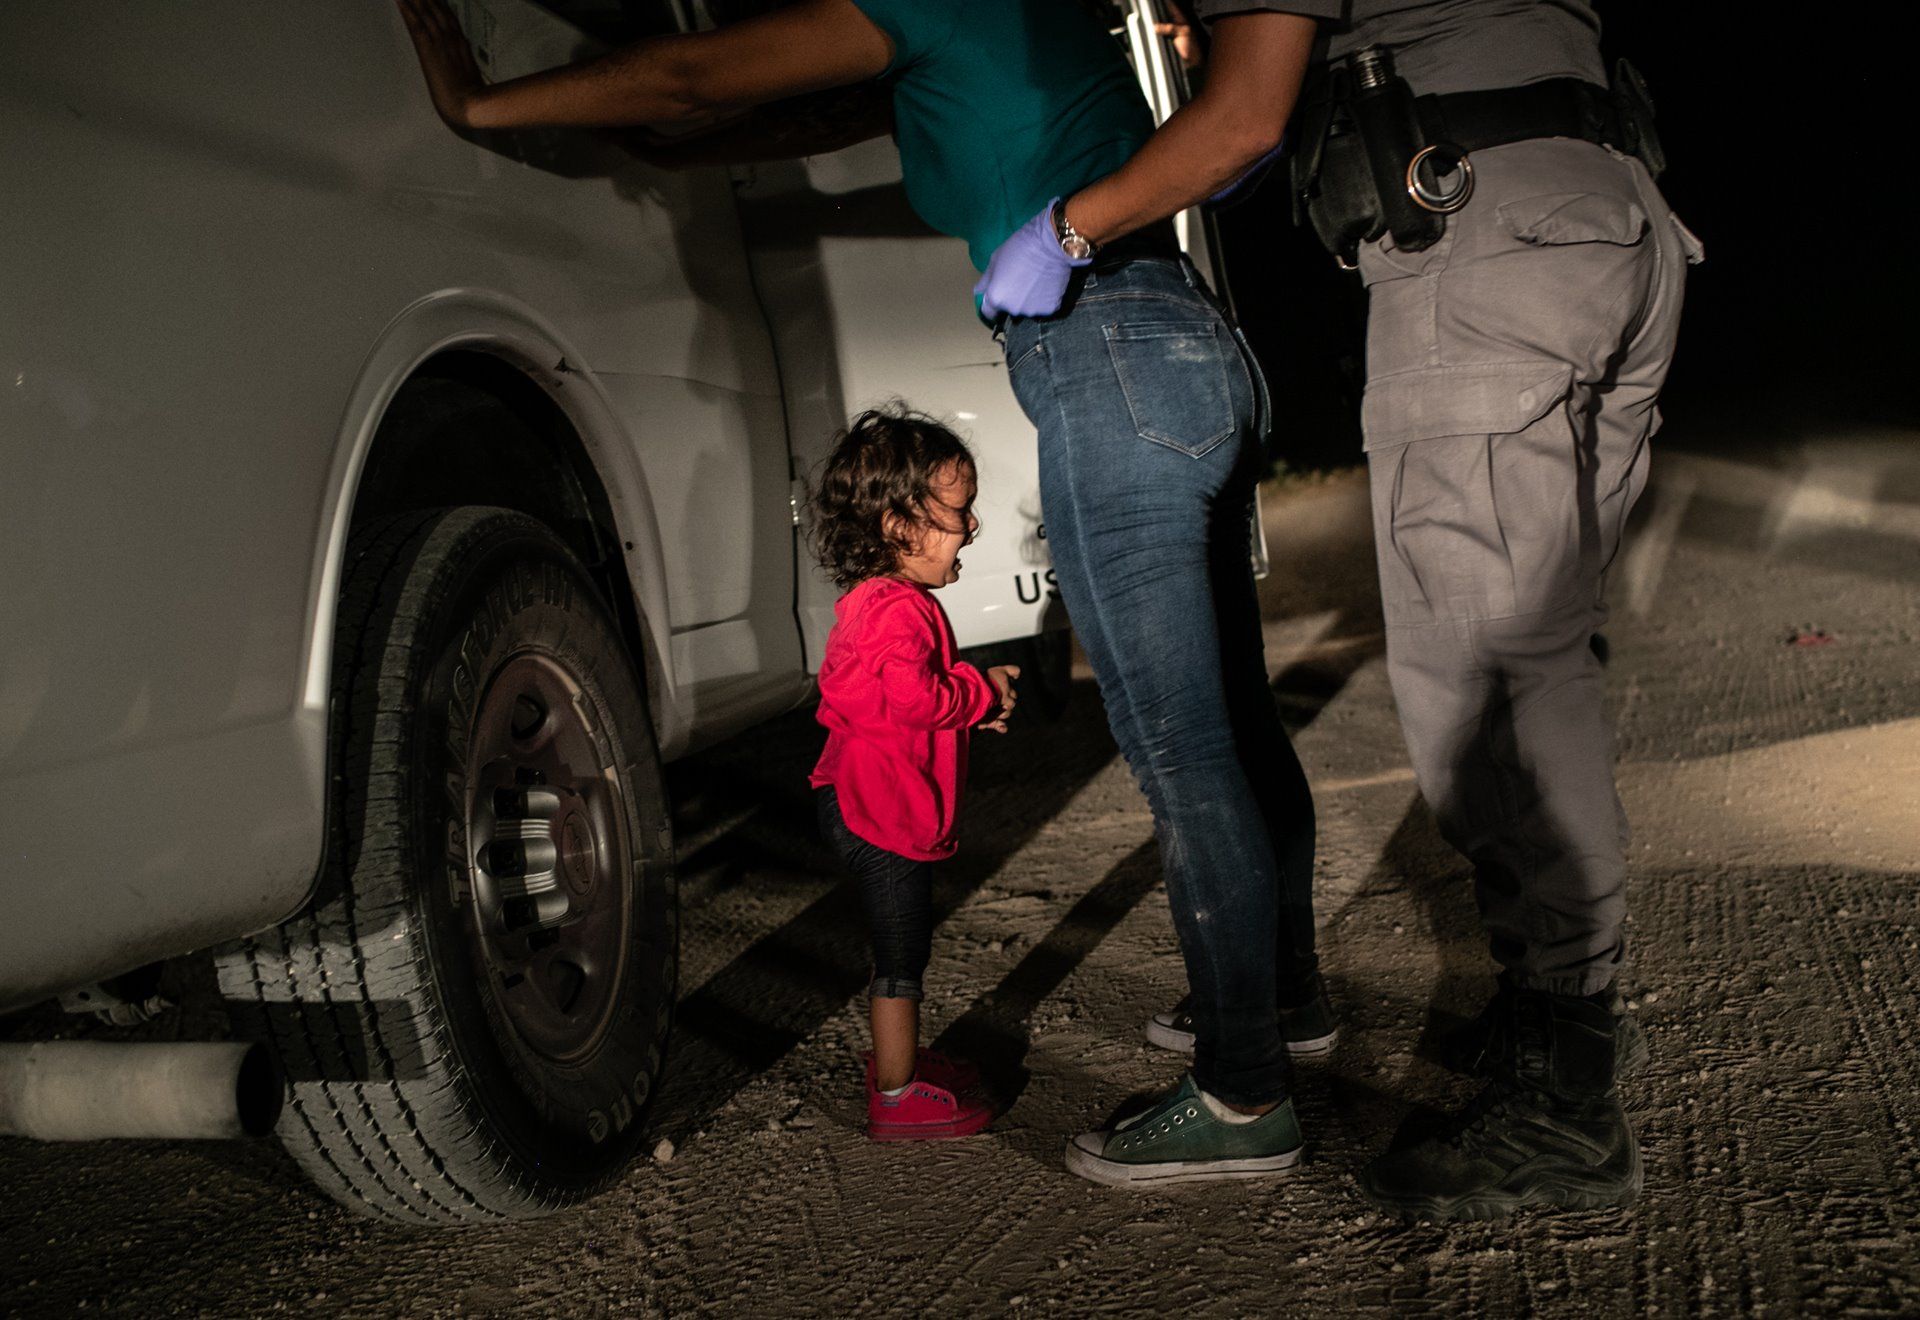
\includegraphics[width=\textwidth,height=\textheight,keepaspectratio]{Images/WPPF-2019PhotoContest-POYNominee-JohnMoore.jpg}
		\caption{{Crying Girl in the Border, John Moore, 18 Junio 2018}}
		\label{fig:foto}

	\end{figure}

	\vspace{0.5cm}

	% TODO: Añadir cita bibliográfica a la imagen 

	\vspace{1cm}
	\hrulefill
\end{titlepage}
\newpage

% NIVEL CONTEXTUAL ____________________________________________________________

En muchas ocasiones demostrar la realidad implica revelar lo que oculta la sociedad detrás de una fachada de irrealidad.

Esto es lo que quiere mostrar el fotógrafo americano John Moore con esta fotografía realizada en junio de 2018, coincidiendo con la nueva política de Trump relacionada con “cero tolerancia” los inmigrantes, siendo procesados como criminales.

Mayoritariamente, esto significaba que los niños eran separados de sus padres, siendo la niña de la foto, Yanela Sánchez, también separada de su madre, Sandra Sánchez, siendo llevada a custodia.

La fotografía se disparó en la frontera de Estados Unidos, más concretamente, en la frontera de McAllen, Texas.\cite{einstein} \newline
% TODO: añadir cita bibliográfica

Podemos definir esta fotografía en el género fotográfico de “prensa” siendo el género más prominente en la fotografía debido a que John Moore es un periodista y fotógrafo para Getty Images.
% TODO: Añadir cita a Getty 

También podemos encontrar otros géneros algo más ocultos, ya que en la fotografía contiene un componente social muy marcado, llamando y criticando como se gestionan los inmigrantes en Estados Unidos de formas inhumanas e irrespetuosas.

Hablando sobre aspectos más técnicos de la imagen, \textit{World Press Photo} nos provee con las características técnicas de la imagen.
La cámara usada fue una Canon EOS-1D X Mark II
% TODO: Conseguir enlace a detalles de cámara 
Una parte muy importante de la fotografía es la sensación de cercanía que otorga la imagen. Se consiguió con objetivo con longitud focal de 35 mm. \\

% NIVEL MORFOLÓGICO ___________________________________________________________

La imagen contiene una gran cantidad de puntualidades que crean una composición bastante cargada, en el que podemos destacar cuatro puntos:
De izquierda a derecha:
\begin{enumerate}
	\item El vehículo.
	\item La niña, más concretamente, su sudadera.
	\item Los pantalones de la madre (y por extensión, la madre.)
	\item Los pantalones del guardia (mismo caso que antes, por extensión, el guardia.)
\end{enumerate}

La fotografía se compone de manera que se incluye a todos los sujetos en el mismo plano. Además, la amplitud del encuadre demuestra ser un plano general en el que no se puede discernir otros elementos fuera de campo. \newline

Siendo una fotografía nocturna y probablemente realizada a prisa y corriendo por el fotógrafo, resulta en una imagen con cierta pérdida de nitidez que podemos achacar a la falta de luz y que la imagen se realizara con valores de ISO relativamente altos. Introduciendo ruido digital en la fotografía y raíz de esto, una pérdida de nitidez. \newline

Aunque, la perdida de la nitidez y la introducción de cierta borrosidad gana en favor de la imagen, creando una sensación de urgencia y confusión que se refleja en la imagen. Probablemente la persona que vea esta imagen le entre le otorgue las características anteriormente mencionadas.  \newline

Como he explicado antes, el hecho de que sea una fotografía nocturna añade el componente de la oscuridad, que en este caso, es un elemento que juega un papel importante en la composición. No obstante, se puede apreciar lo que parece unos faros de un vehículo (\textit{probablemente luces de carretera}), este detalle significa que es posible que haya otras personas fuera de campo que no podemos ver. 
En términos más técnicos, la iluminación es artificial con un balance entre dura y suave. El hecho de que al ser de noche y que las luces provengan de un ángulo de 90º, se crea un balance entre las claves altas (\textit{el hecho de haya una luz muy fuerte}) y la clave baja (\textit{la misma luz crea muchas sombras que se aprecian en el fondo de la composición})  \newline

% TODO: Quizás puedo añadir otra cita bibliográfica?

Otro elemento muy fuerte en esta imagen es el brutal contraste que existe, no entre las luces u otros elementos; sino en la ropa que llevan las personas de la fotografía. La niña destaca prácticamente sobre todo lo demás que rodea a la fotografía, con su ropa roja; además de estar justo delante de una camioneta blanca añadiendo todavía más contraste a la niña haciéndola destacar todavía más. 

Esto también ocurre con la madre, pero a un nivel menos elevado, sus pantalones también resaltan al estar delante de la puerta blanca de la camioneta. \newline

% NIVEL COMPOSITIVO ___________________________________________________________



% NIVEL ENUNCIATIVO ___________________________________________________________



\newpage

% Bibliografia  _______________________________________________________________
\printbibliography
\newpage

\blinddocument
\end{document}